\begin{comment}
To Do:
\begin{itemize}
\color{red}
     \item Define the specific goals of the study, e.g., which characteristics of the problem will be used to assess the validity of the proposed solution?
     \item Design an empirical strategy to address the specific goals established.
    \item The pipeline implemented must be shown to work on a non-trivial (possibly real-world) example— a toy problem is not admitted.
    \item The pipeline implemented is experimented using a dataset with 3D images.
    \item A comprehensive analysis of multiple performance indicators.
    \item Implementation of the user feedback mechanism.
\end{itemize}

\begin{enumerate}
\color{blue}
\item \textbf{Preprocessing:} Explain the steps taken to preprocess the images, such as resizing, cropping, and normalization. Also, mention any techniques used to address issues like noise or distortion in the images.
\item \textbf{Feature Extraction:} Outline the techniques used to extract features from the images. This could include handcrafted features or deep learning approaches such as convolutional neural networks.
\item \textbf{Modeling:} Explain the algorithm used to build the model for emotional recognition in images, including any modifications made to the model architecture or hyperparameters.
\item \textbf{Evaluation:} Describe the evaluation metrics used to assess the performance of the model, such as accuracy, precision, recall, or F1-score. Also, mention the cross-validation approach used to ensure the generalization of the model.
\item \textbf{Comparison with Previous Studies:} Compare the results of your model with those of previous studies on emotional recognition in images, if any.
\item \textbf{Ethical Considerations:} Discuss the ethical considerations related to the use of image data, such as ensuring the privacy and confidentiality of the participants in the dataset.
\item \textbf{Limitations and Future Work:} Mention the limitations of your study and outline the future work that can be done to improve the emotional recognition in images.
\end{enumerate}
\end{comment}

\begin{figure}[h!]
\centering
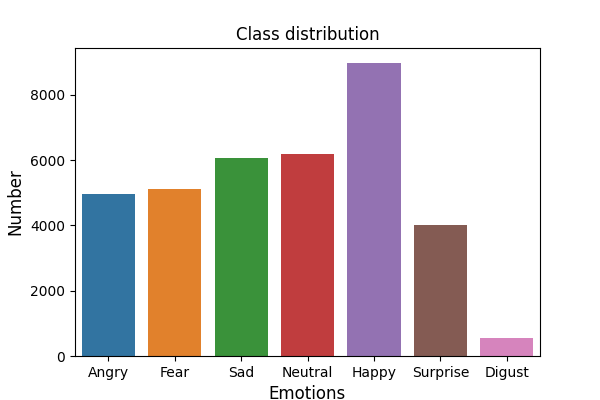
\includegraphics[scale=0.8]{barplot1.png}
\caption{Barplot of the distribution of the different classes of emotion.}\label{fig:emo-distribution}
\end{figure}

\begin{enumerate}
\item \textbf{Data Collection:} %The fer2013 dataset is handled according to the terms of the Open Database License (ODbL), which states the following: "The Licensor grants to You a worldwide, royalty-free, non-exclusive, perpetual, irrevocable copyright license to do any act that is restricted by copyright over anything within the Contents, whether in the original medium or any other. These rights explicitly include commercial use, and do not exclude any field of endeavour. These rights include, without limitation, the right to sublicense the work." \cite{odbl} We may use additional datasets provided by kaggle or other sources. 

To recognize emotions in images, the kaggle dataset \textbf{FER2013} \cite{FER2013} will be used. This dataset was prepared by Pierre-Luc Carrier and Aaron Courville as part of an ongoing research project and contains $35,887$ images, displaying the emotions anger, fear, sadness, neutralilty, happiness, surprise and disgust. Hereby, \ref{fig:emo-distribution} represents the corresponding distribution of those emotions. Moreover, this dataset includes people from different genders, ethnicities and ages. Furthermore, the FER2013 dataset is handled according to the terms of the Open Database License (ODbL), which states the following: ``The Licensor grants to You a worldwide, royalty-free, non-exclusive, perpetual, irrevocable copyright license to do any act that is restricted by copyright over anything within the Contents, whether in the original medium or any other. These rights explicitly include commercial use, and do not exclude any field of endeavour [...].'' \cite{odbl} We may also use additional datasets provided by kaggle or other sources.

\begin{figure}[h]
\centering
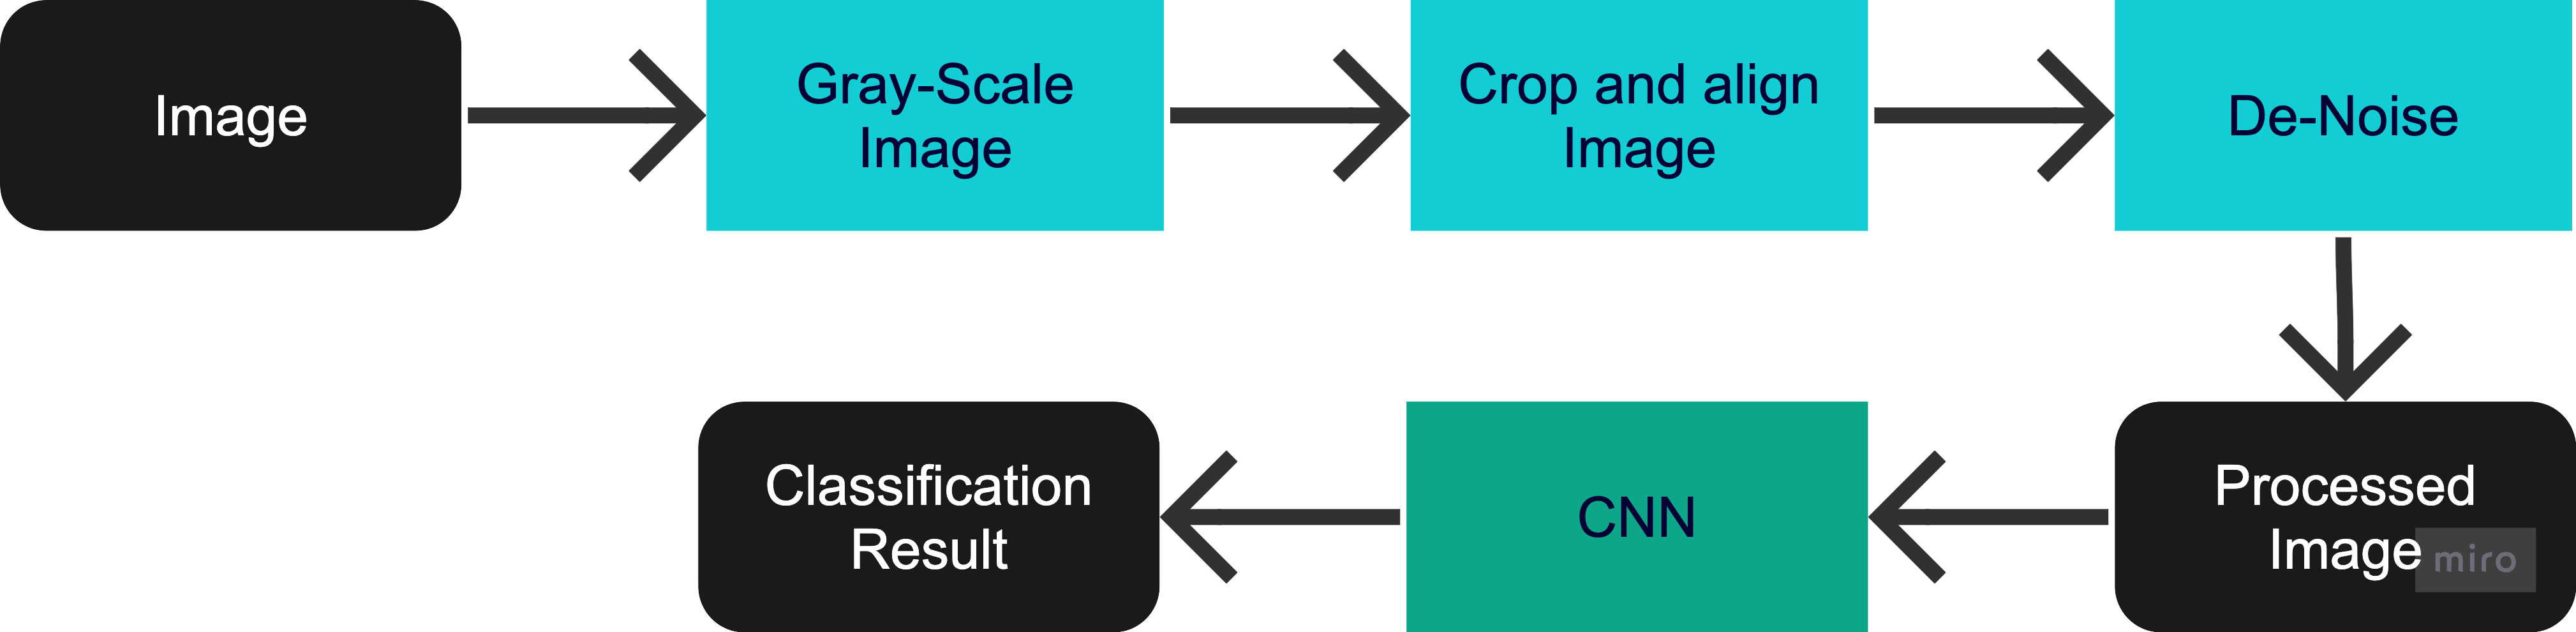
\includegraphics[width=0.9\textwidth]{images/fer-preprocessing-modelling.png}
\caption{Preprocessing and Modeling.}\label{fig:prep-mod}
\end{figure}

\item \textbf{Preprocessing:}
Before using the datasets, they will be preprocessed to exclude irrelevant images/emotions. Data preprocessing includes reducing different types of noises, resizing the picture and aligning facial features. The method typically used to achieve the results is the eye selection method. Figure \ref{fig:emo-distribution} provides an example image of the different facial expressions with there corresponding labeled emotion. 
The \textit{FER2013} dataset provides preprocessed and labeled grayscaled images of facial emotions. We will however implement a pipeline to process new images. This will contain the following steps. The fist step is to convert the (RGB) color image to a grayscale image. The colors in images can often contain clutter and  hinder the model form detecting faces accurately. After the grayscale conversion, the next step is to crop and align the images, so that we are left only with the face. We should mention, that in this step we have to consider the resolution of the image and if the crop is still usable after the crop. The next step is to de-noise the image and apply filtering. De-noising the image will amplify and enhance meaningful features of an image, while reducing background noise.   Filtering is the process of altering properties of the image, for example contrast and saturation.

\item \textbf{Modeling:}
Afterwards, a CNN with 2D convolutional layers will be used. This approach has been shown to be effective for image recognition tasks. We will experiment with the layers and parameters to try to achieve the best possible results. 

\begin{figure}[h]
\centering
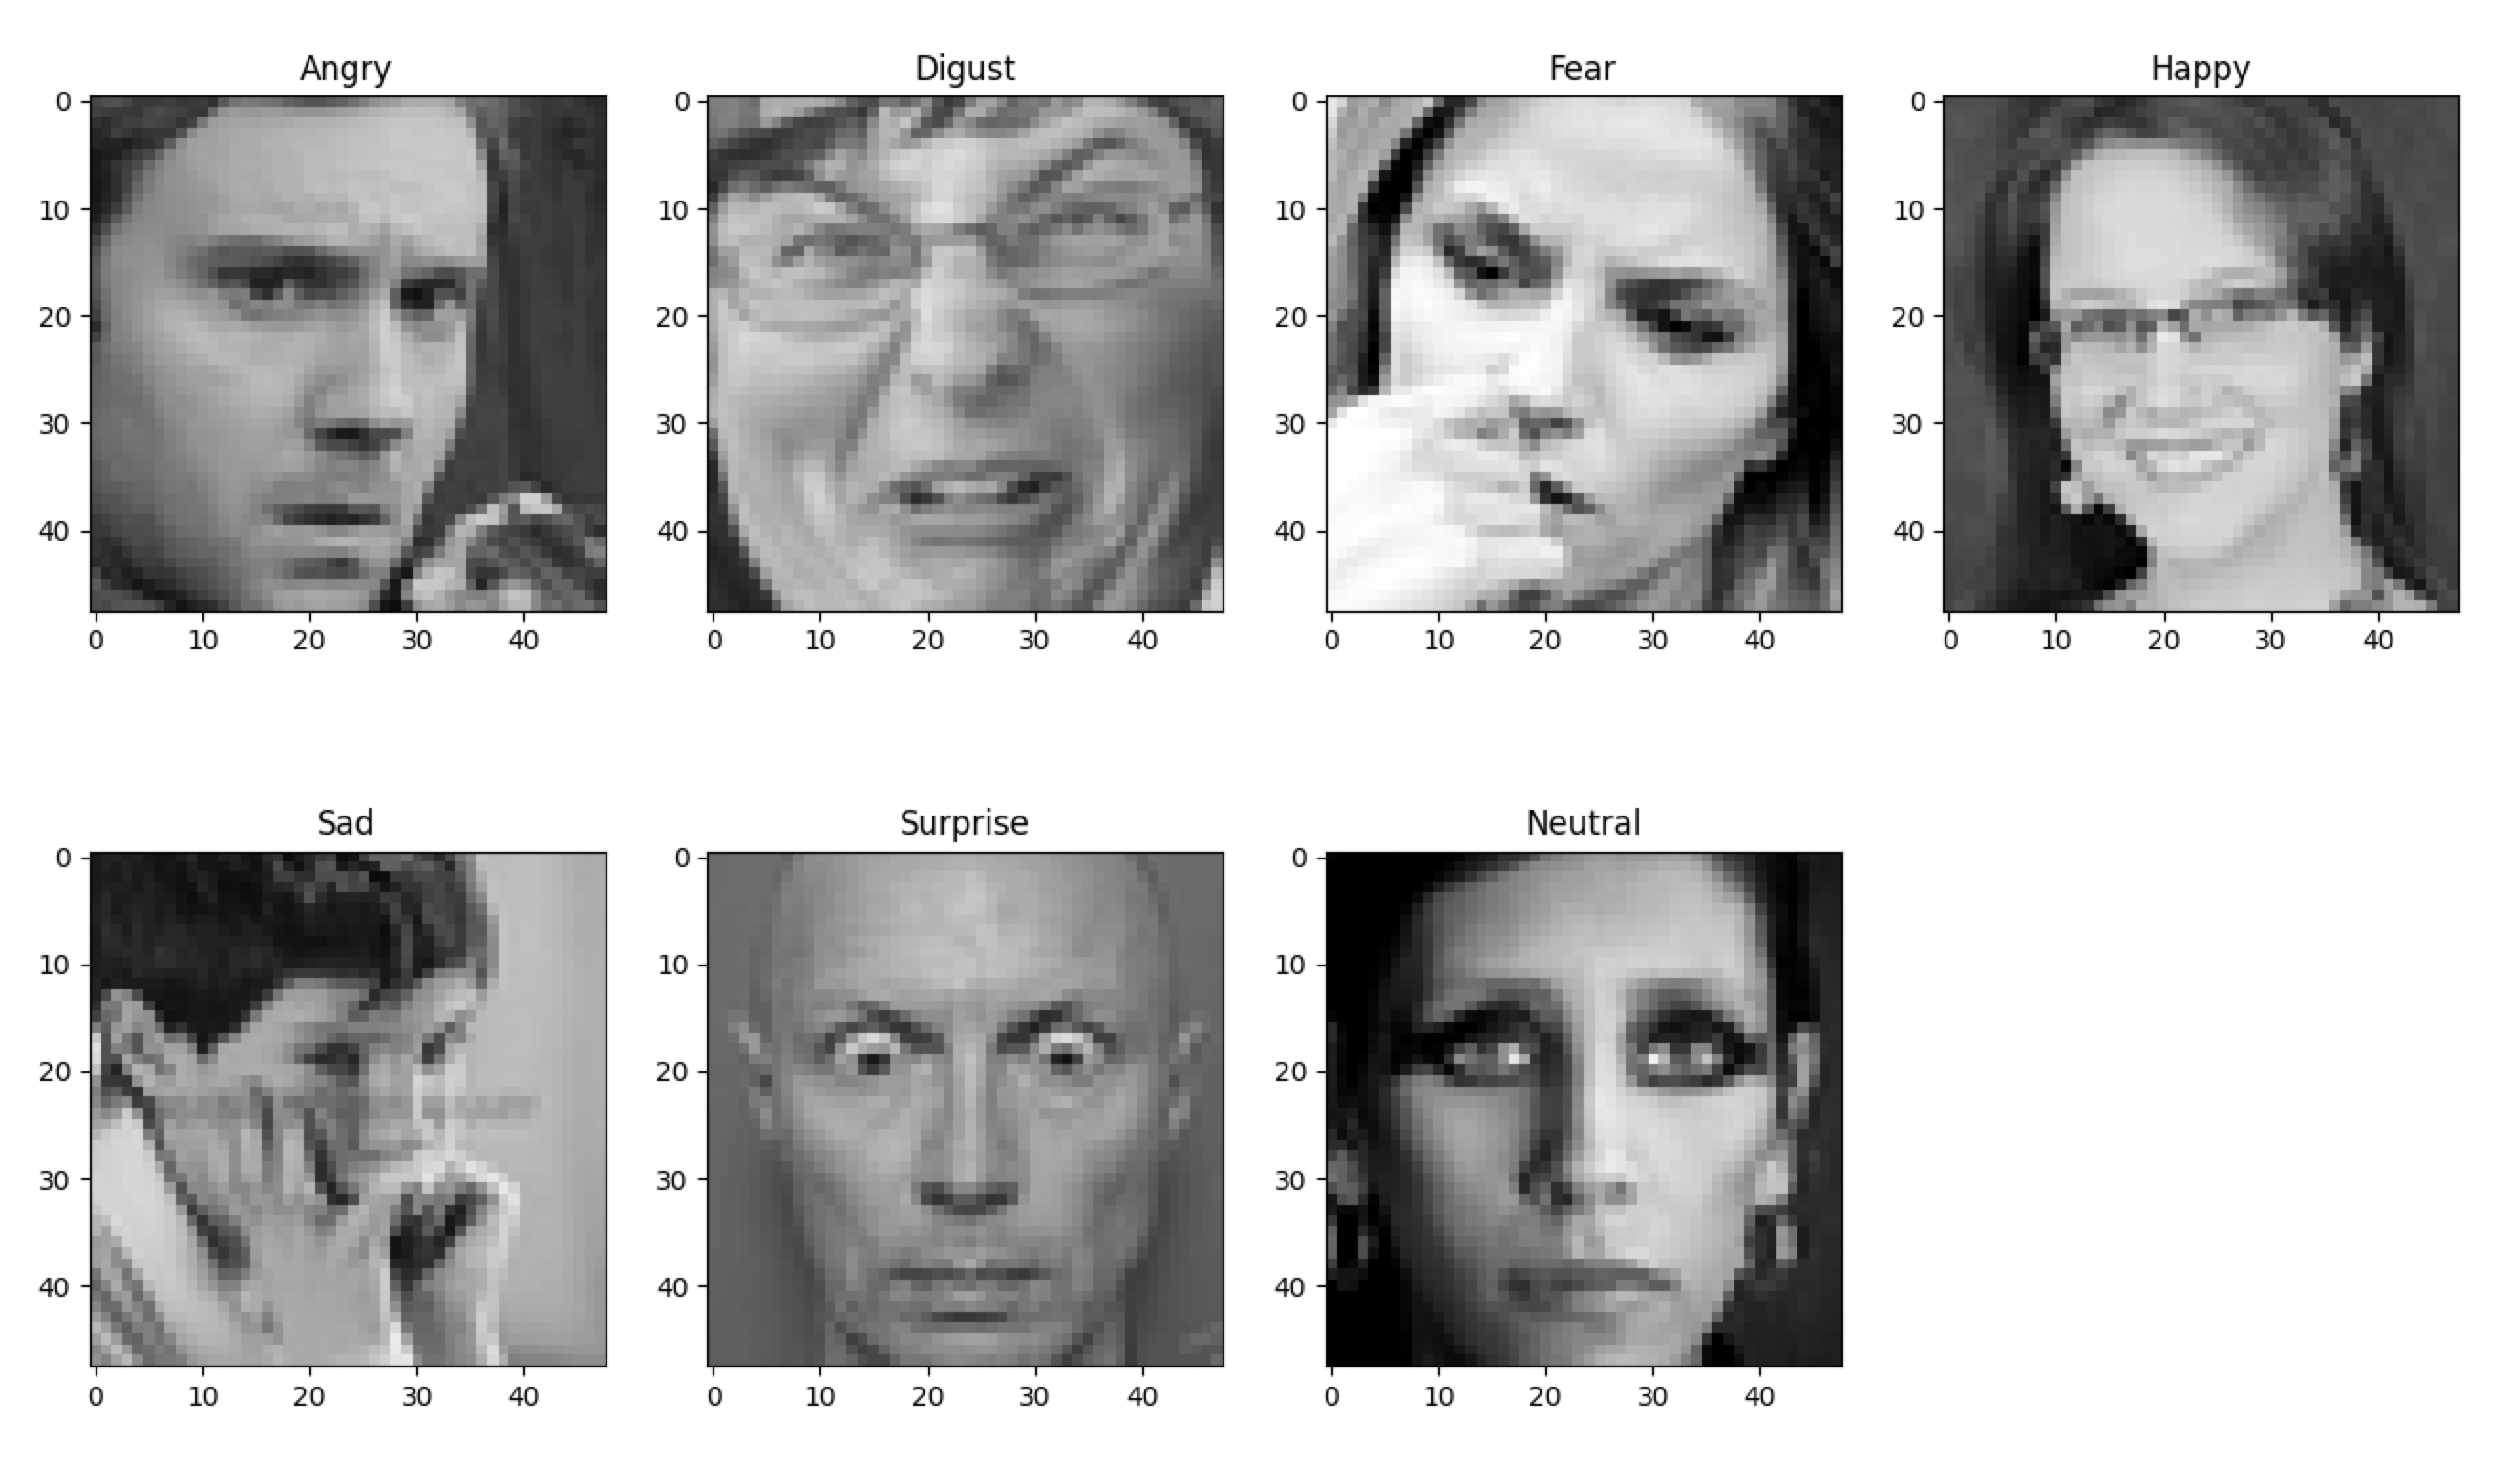
\includegraphics[width=0.9\textwidth]{faces1.png}\\
\caption{Facial expressions with corresponding emotions. \cite{FER2013}}\label{fig:faces}
\end{figure}

\newpage
\item \textbf{Model Evaluation:}
After training a model, the next goal is to test the model on new data. For this we can firstly use the test data and measure the accuracy, precision and recall. However for more practical applications our goal would be to implement an image preprocessing pipeline to allow us to apply the trained model on real-world captured images. This can then in turn be applied to frames of a video evaluating the emotions of one person (possibly multiple people if feasible). This will also preform as an alternative to the classic metrics for quality assurance, by allowing the person captured on the image to input their actual emotion and comparing their actual emotion to the predicted one. If we collect the new labeled images that were imputed by a user, we can retrain the model with more data, if the accuracy drops below a predetermined threshold.

\begin{figure}[h]
\centering
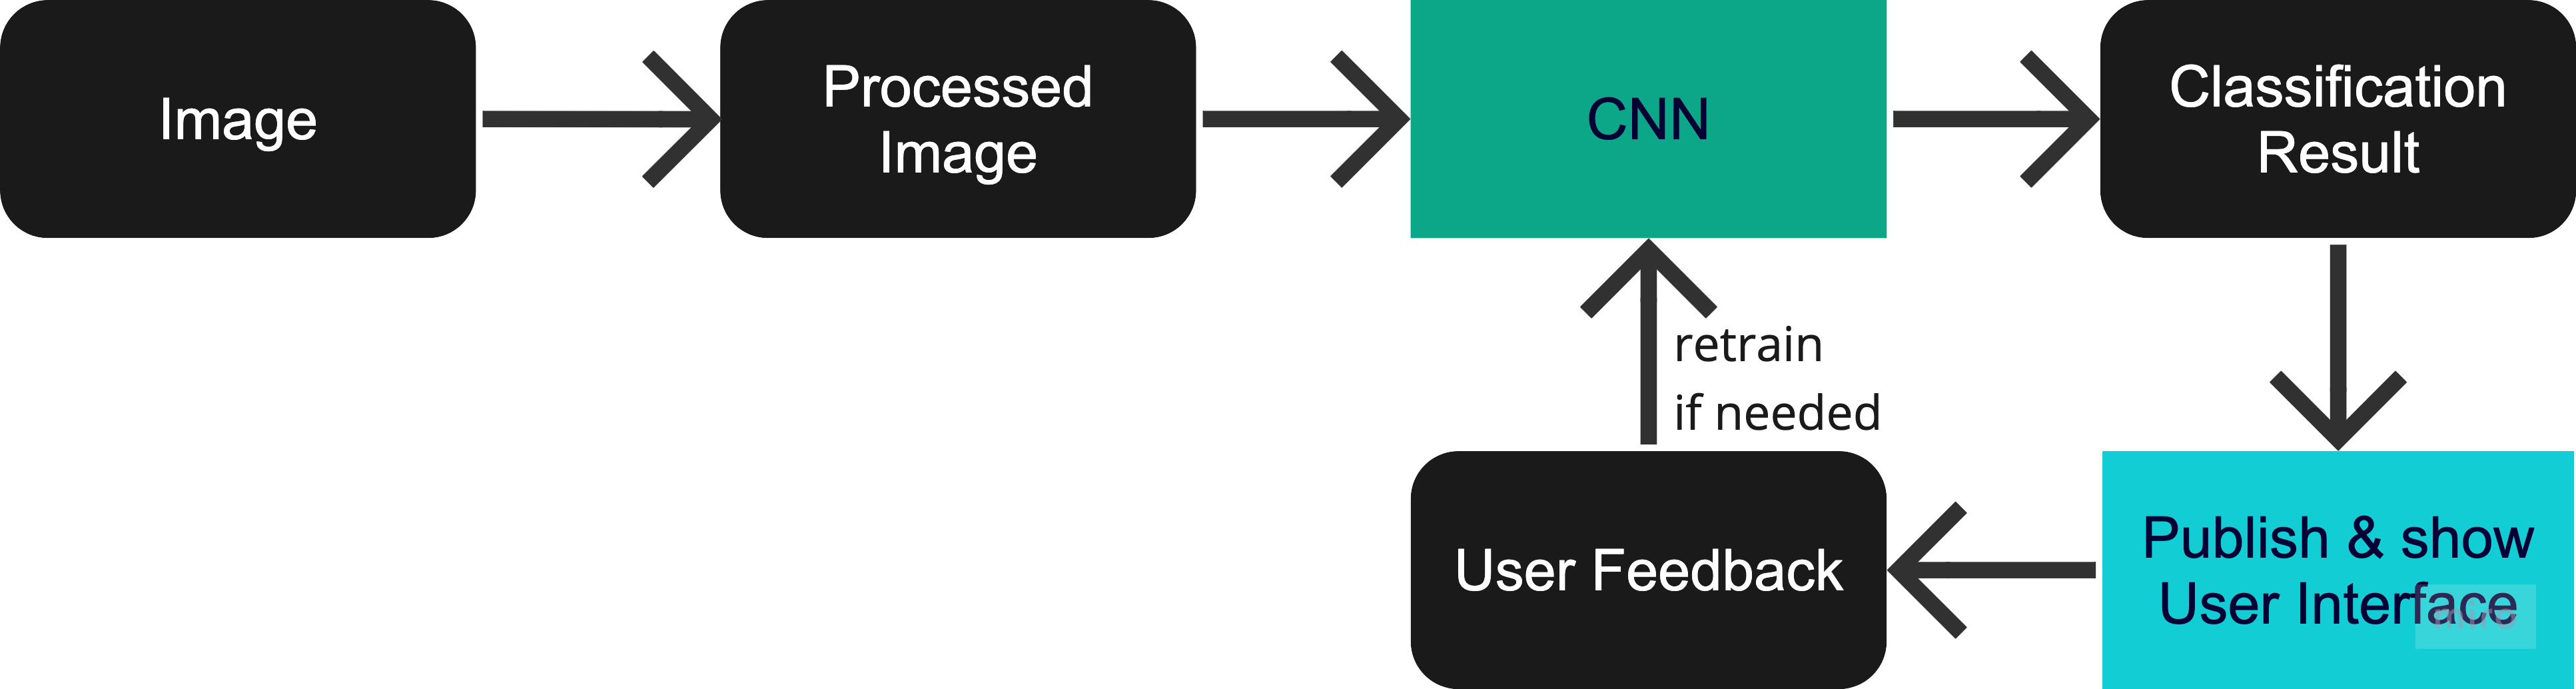
\includegraphics[width=0.9\textwidth]{images/fer-user-feedback.png}\\
\caption{General overview of the \acrshort{fer} system and user feedback}\label{fig:userfb}
\end{figure}

\end{enumerate}
\newpage

\begin{comment}
    \noindent We will implement the following files, containing classes for different models, data processing and tests: 
    \begin{enumerate}
        \item main.py
        \item ann\_model.py
        \item dataprocessing.py
        \item tests.py
    \end{enumerate}
    
    To address:
    \begin{itemize}
    \color{blue}
        \item Basic interface to better define the use case of the trained model. 
        \item Model Training: Train a deep neural network model using the preprocessed dataset.
        \item Model Evaluation: Evaluate the trained model using various metrics such as accuracy, precision, and recall.
        \item Get an Accuracy of around 65\% 
        \item System Development: Develop the emotional recognition system using the trained model and
        software engineering principles such as modular design, testing, and documentation.
        \item System Evaluation: Evaluate the developed system using various metrics such as performance, scalability, and maintainability.
        \item User Feedback: Incorporate user feedback mechanisms to improve the system’s accuracy and adaptability to new scenarios.
        \item Continuous datastreams (i.e. Video)
        \item Visualisation (Graphs, Barplots, ...) 
    \end{itemize}
\end{comment}

%\section{Preliminary results and findings}
%\section{Implications of the results}